\apendice{Especificación de diseño}

\section{Introducción}

En este apéndice vamos a hablar sobre los diferentes aspectos de diseño.

\section{Diseño de datos}

En este proyecto se trabaja con muchos datos, pero la mayoría de ellos son del mismo tipo. Se trabaja con gran cantidad de Strings o cadenas de caracteres. La lógica de trabajar con cadenas de caracteres frente a otros tipos de datos radica en la facilidad para ser leídos a través de un \textit{buffer} o incluso de ser tratados. Además, hay que tener en cuenta que ciertos tipos de datos no pueden ser almacenados o enviados. Por ejemplo, en nuestra base de datos querríamos almacenar el estado de las luces mediante una variable de tipo \verb|boolean|, pero nuestra base de datos \textbf{Sqlite} no permite alamcenarlos. En su defecto, el estado de las luces ha tenido que ser guardado mediante una variable de tipo \verb|Integer| que podrá contener los valores \textit{0} o \textit{1}.

En nuestra base de datos, ya sea en la parte de Raspberry Pi o de Android, solo almacenaremos cadenas de caracteres (\verb|Strings|) o números (\verb|Integer|). A través de la conexión entre clientes y servidor solo se manda cadenas de caracteres a través de un \textit{buffer} para realizar cambios en cualquiera de las partes. Solamente se ha hablado de estos dos tipos de datos porque son los dos únicos tipos que o se almacenan para su tratamiento o son tratados en el momento.

\section{Diseño procedimental}

\begin{figure}[h!]
	\centering
	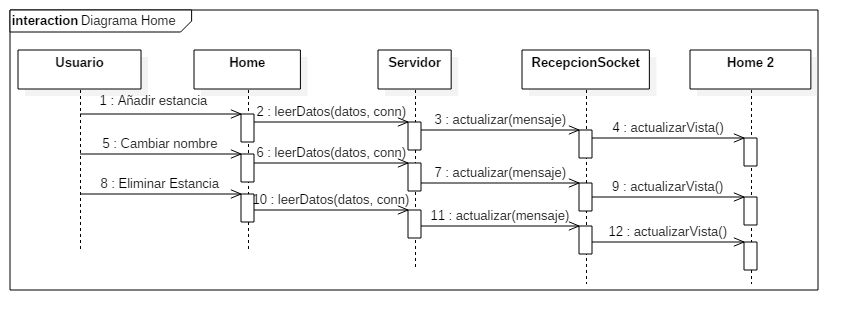
\includegraphics[width=1.2\linewidth]{img/DiagramaHome}
	\caption{Diagrama de acciones sobre una estancia en la clase \textbf{Home}.}
	\label{fig:DiagramaHome}
\end{figure}

\begin{figure}[h!]
	\centering
	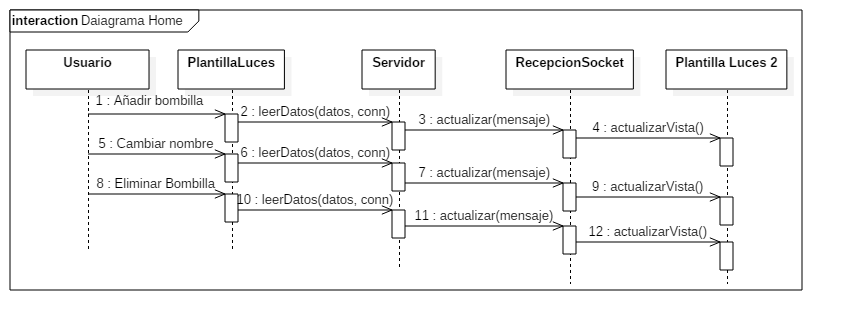
\includegraphics[width=1.2\linewidth]{img/DiagramaPlantillaLuces}
	\caption{Diagrama de acciones sobre una bombilla en la clase \textbf{PlantillaLuces}.}
	\label{fig:DiagramaPlantillaLuces}
\end{figure}

\section{Diseño arquitectónico}

En este apartado hablaremos del diseño arquitectónico de ambas partes del proyecto.

\subsection{Raspberry Pi}

En esta parte del proyecto no existen paquetes que agrupen los ficheros y los archivos se encuentran en la raíz del proyecto. Vamos a hablar brevemente de los métodos y características de estos ficheros.

\subsubsection{Servidor.py}

En este fichero se encuentra la implementación de la clase \textit{Servidor} que contiene los siguientes métodos.

\begin{itemize}
	\item \verb|__init__(self)|: se encarga de inicializar las variables, iniciar la interfaz y arrancar el servidor en un hilo independiente.
	\item \verb|iniciarInterfaz(self)|: se encarga de inicializar todas la variables y estructuras de la interfaz y arrancarla.
	\item \verb|centrarVentana(self, ventana, widht, height)|: centra la ventana pasada por parámetro con un tamaño igual a \textit{widht} y \textit{height}.
	\item \verb|agregarIp(self)|: se encarga de mostrar una nueva ventana desde la que poder actualizar la IP.
	\item \verb|actualizarIp(self)|: se encarga de recoger el valor de la IP que se ha introducido en la ventana creada por \verb|agregarIp(self)|.
	\item \verb|leerDatos(self, datos, conn)|: se encarga de interpretar todos los mensajes que llegan al servidor y actuar en medida de lo que se ha leído.
	\item \verb|clienteThread(self, conn)|: se encarga de crear un nuevo hilo independiente para cada conexión de un cliente con el servidor.
	\item \verb|iniciarServidor(self)|: se encarga de inicializar todas las variables y estructuras del servidor y arrancarlo.
	\item \verb|main()|: se encarga de realizar la ejecución principal del archivo.
\end{itemize}

\subsubsection{Database.py}

En este fichero se encuentra la implementación de la clase \textit{Database} que contiene los siguiente métodos

\begin{itemize}
	\item \verb|__init__(self)|: se encarga de crear las tablas de la base de datos si no estuviesen ya creadas.
	\item \verb|insertarEstancia(self, id, nombre)|: se encarga de insertar una nueva estancia en la base de datos.
	\item \verb|insertarElemento(self, estancia, nombre, estado)|: se encarga de insertar un nuevo elemento en la base de datos.
	\item \verb|actualizarEstancia(self, nombreViejo, nombreNuevo)|: se encarga de actualizar el nombre de una estancia de la base de datos.
	\item \verb|actualizarElemento(self, estancia, nombreViejo, nombreNuevo)|: se encarga de actualizar nombre de un elemento de una estancia de la base de datos.
	\item \verb|actualizarEstado(self, estancia, nombre, estado)|: se encarga de actualizar el estado de un elemento de una estancia de la base de datos.
	\item \verb|actualizarIP(self, ip)|: se encarga de actualizar la IP de la base de datos.
	\item \verb|eliminarEstancia(self, estancia)|: se encarga de eliminar una estancia de la base de datos.
	\item \verb|eliminarElemento(self, estancia, index)|: se encarga de eliminar un elemento de una estancia de la base de datos.
	\item \verb|recuperarEstancia(self, index)|: se encarga de devolver una estancia de la base de datos.
	\item \verb|recuperarElemento(self, estancia, index)|: se encarga de devolver un elemento de la base de datos.
	\item \verb|recuperarIp(self)|: se encarga de devolver la ip almacenada en la base de datos.
	\item \verb|numeroEstancias(self)|: se encarga de devolver el número de estancias en la base de datos.
	\item \verb|numeroElementos(self, estancia)|: se encarga de devolver el número de elementos de una estancia de la base de datos.
	\item \verb|cerrarBD(self)|: se encarga de cerrar la conexión con la base de datos.
	\item \verb|borrarBD(self)|: se encarga de borrar todas las tablas de la base de datos.
\end{itemize}

\subsubsection{Aplicación Android}

En esta parte del proyecto no existen paquetes para diferenciar unas clases de otras, todas se encuentran en el directorio \textbf{Simulador Domotica Raspberry/app android/app/src/main/java/mario/app android}. La función de cada una de las clases la podemos encontrar en la sección \ref{sec:explicacionAndroid}. Aquí simplemente vamos a visualizar el diagrama de clases de cada uno de los ficheros \textit{.java} de ese directorio.

\begin{enumerate}
	\item \verb|BDLocal|: \ref{fig:BDLocal}
	\begin{figure}[h!]
		\centering
		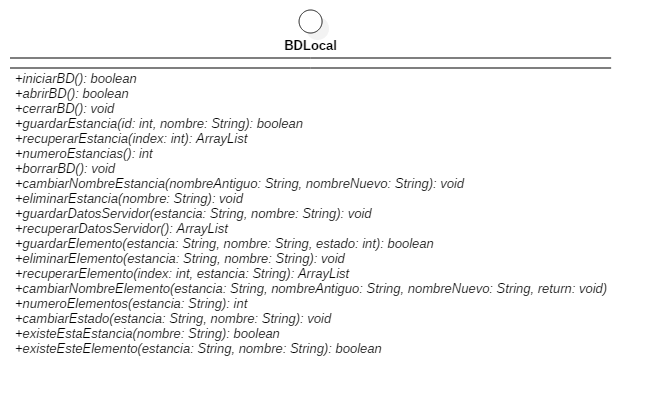
\includegraphics[width=1.1\linewidth]{img/BDLocal}
		\caption{Diagrama de la clase \textbf{BDLocal}.}
		\label{fig:BDLocal}
	\end{figure}
	\item \verb|SQLite|: \ref{fig:SQLite}
	\begin{figure}[h!]
		\centering
		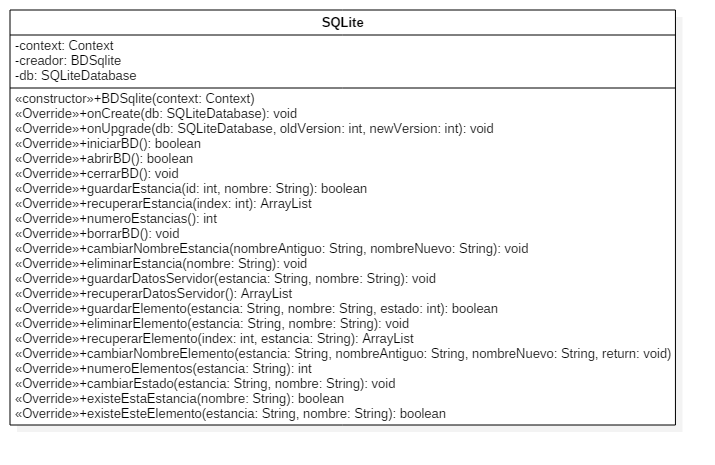
\includegraphics[width=1.1\linewidth]{img/SQLite}
		\caption{Diagrama de la clase \textbf{SQLite}.}
		\label{fig:SQLite}
	\end{figure}
	\item \verb|Conexion|: \ref{fig:Conexion}
	\begin{figure}[h!]
		\centering
		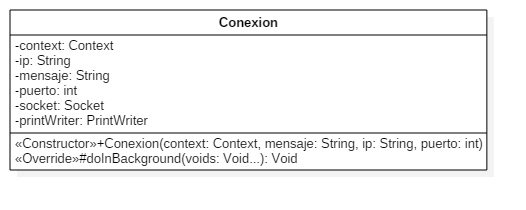
\includegraphics[width=1.1\linewidth]{img/Conexion}
		\caption{Diagrama de la clase \textbf{Conexion}.}
		\label{fig:Conexion}
	\end{figure}
	\item \verb|CustomAdapterEstancia|: \ref{fig:CustomAdapterEstancia}
	\begin{figure}[h!]
		\centering
		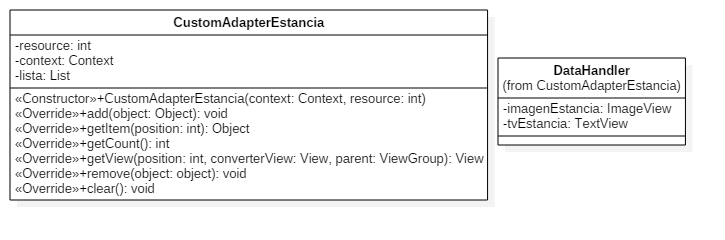
\includegraphics[width=1.2\linewidth]{img/CustomAdapterEstancia}
		\caption{Diagrama de la clase \textbf{CustomAdapterEstancia}.}
		\label{fig:CustomAdapterEstancia}
	\end{figure}
	\item \verb|CustomAdapterLuz|: \ref{fig:CustomAdapterLuz}
	\begin{figure}[h!]
		\centering
		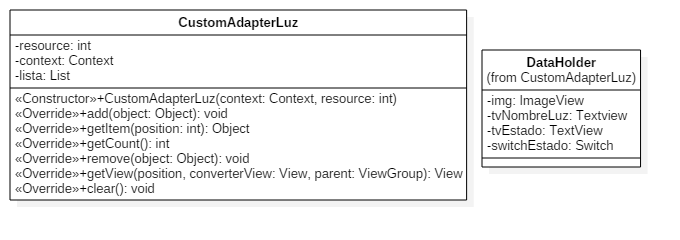
\includegraphics[width=1.3\linewidth]{img/CustomAdapterLuz}
		\caption{Diagrama de la clase \textbf{CustomAdapterLuz}.}
		\label{fig:CustomAdapterLuz}
	\end{figure}
	\item \verb|Habitacion|: \ref{fig:Habitacion}
	\begin{figure}[h!]
		\centering
		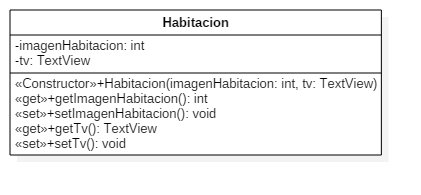
\includegraphics[width=1\linewidth]{img/Habitacion}
		\caption{Diagrama de la clase \textbf{Habitacion}.}
		\label{fig:Habitacion}
	\end{figure}
	\item \verb|Home|: \ref{fig:Home}
	\begin{figure}[h!]
		\centering
		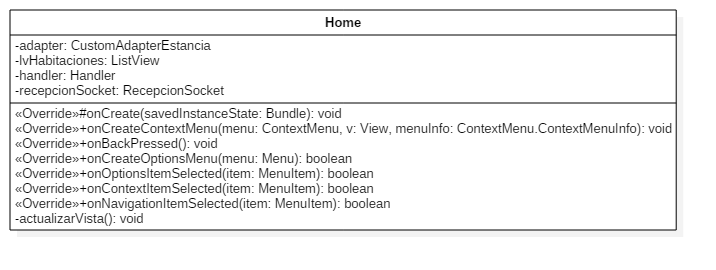
\includegraphics[width=1.2\linewidth]{img/Home}
		\caption{Diagrama de la clase \textbf{Home}.}
		\label{fig:Home}
	\end{figure}
	\item \verb|Luz|: \ref{fig:Luz}
	\begin{figure}[h!]
		\centering
		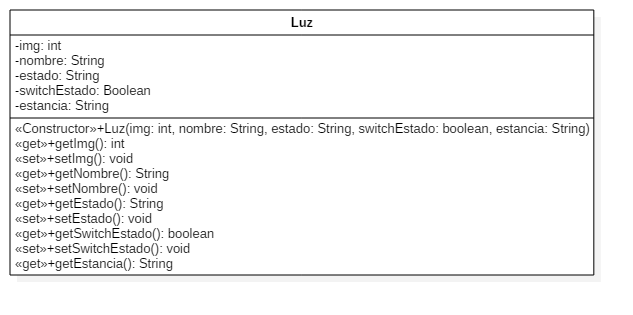
\includegraphics[width=1.2\linewidth]{img/Luz}
		\caption{Diagrama de la clase \textbf{Luz}.}
		\label{fig:Luz}
	\end{figure}
	\item \verb|PlantillaLuces|: \ref{fig:PlantillaLuces}
	\begin{figure}[h!]
		\centering
		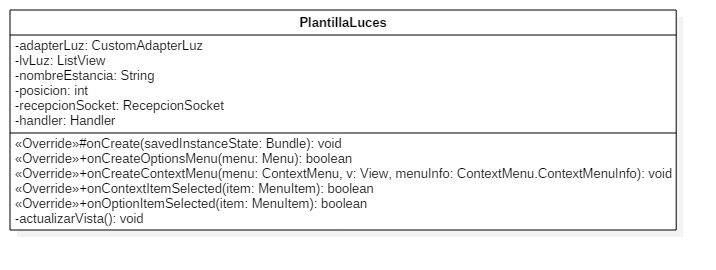
\includegraphics[width=1.3\linewidth]{img/PlantillaLuces}
		\caption{Diagrama de la clase \textbf{PlantillaLuces}.}
		\label{fig:PlantillaLuces}
	\end{figure}
	\item \verb|RecepcionSocket|: \ref{fig:RecepcionSocket}
	\begin{figure}[h!]
		\centering
		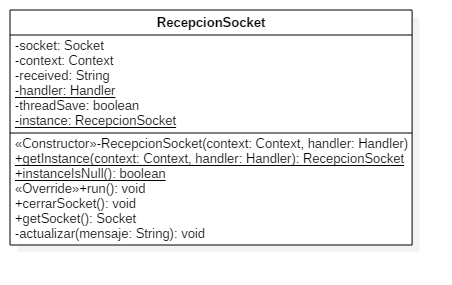
\includegraphics[width=1\linewidth]{img/RecepcionSocket}
		\caption{Diagrama de la clase \textbf{RecepcionSocket}.}
		\label{fig:RecepcionSocket}
	\end{figure}
	\item \verb|Servidor|: \ref{fig:DiagramaServidor}
	\begin{figure}[h!]
		\centering
		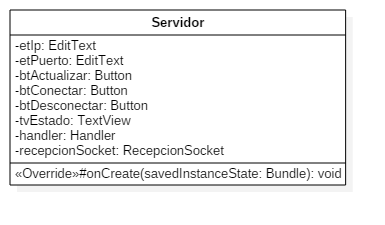
\includegraphics[width=0.9\linewidth]{img/DiagramaServidor}
		\caption{Diagrama de la clase \textbf{Servidor}.}
		\label{fig:DiagramaServidor}
	\end{figure}
\end{enumerate}